\subsection{Observer}
\subsubsection{Định nghĩa}
Observer là một mẫu thiết kế hành vi trong đó có một đối tượng chủ đạo (subject) duy trì danh sách các đối tượng quan sát (observers) và thông báo cho chúng về bất kỳ sự thay đổi nào trong trạng thái của nó. Điều này cho phép các đối tượng quan sát tự động cập nhật khi có sự thay đổi xảy ra.
\subsubsection{Cách sử dụng}
Ta sẽ sử dụng mẫu Pattern trên trong các trường hợp sau:
\begin{itemize}
    \item Sự thay đổi trạng thái ở 1 đối tượng cần được thông báo đến các đối tượng khác mà không phải giữ chúng liên kết quá chặt chẽ.
    \item Khi thay đổi một đối tượng yêu cầu việc thay đổi đến các đối tượng khác, và bạn không biết số lượng đối tượng cần thay đổi.
    \item Khi bạn muốn giảm sự phụ thuộc giữa các đối tượng và cho phép chúng hoạt động độc lập với nhau.
\end{itemize}
\subsubsection{Cấu trúc}
\begin{center}
    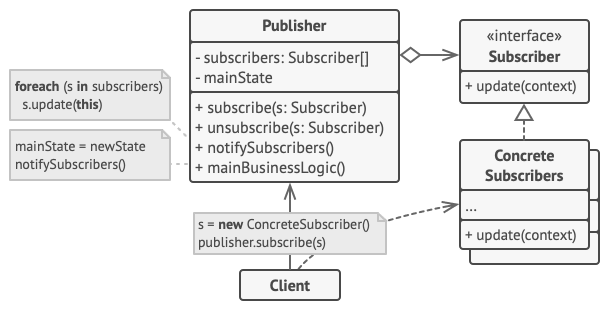
\includegraphics[scale= 0.6]{image/behavioral/observer.png}
\end{center}
\subsubsection{Ưu điểm và Nhược điểm}
Có các ưu điểm và nhược điểm sau:
Ưu điểm:
\begin{itemize}
    \item Sự thay đổi trạng thái ở 1 đối tượng có thể được thông báo đến các đối tượng khác mà không phải giữ chúng liên kết quá chặt chẽ.
    \item Không giới hạn số lượng Observer
    \item Đảm bảo sự tương tác giữa các đối tượng không phụ thuộc: Subject và observers không biết gì về sự tồn tại của nhau, do đó, chúng có thể hoạt động một cách độc lập và tái sử dụng được.
\end{itemize}
Nhược điểm:
\begin{itemize}
    \item Khi có nhiều observers và có nhiều thông báo được gửi đi, quá trình thông báo có thể gây ra sự chậm trễ và ảnh hưởng đến hiệu năng của hệ thống.
    \item Bởi vì các Observer không biết về sự hiện diện của nhau, nó có thể gây tốn nhiều chi phí của việc thay đổi Subject.
\end{itemize}
\subsubsection{Code Example}
\begin{itemize}
    \item Có interface Observer, Display là subclass có hàm update để cập nhật trạng thái.
    \item Có class WeatherStation.
\end{itemize}
\begin{lstlisting}
#include <iostream>
#include <vector>
#include <algorithm>

// Observer interface
class Observer {
public:
    virtual void update(int temperature) = 0;
};

// Subject class
class WeatherStation {
private:
    int temperature;
    std::vector<Observer*> observers;

public:
    void attach(Observer* observer) {
        observers.push_back(observer);
    }

    void detach(Observer* observer) {
        auto it = std::find(observers.begin(), observers.end(), observer);
        if (it != observers.end()) {
            observers.erase(it);
        }
    }

    void setTemperature(int newTemperature) {
        temperature = newTemperature;
        notify();
    }

    void notify() {
        for (auto observer : observers) {
            observer->update(temperature);
        }
    }
};

// Concrete Observer class
class Display : public Observer {
public:
    void update(int temperature) {
        std::cout << "Temperature changed: " << temperature << std::endl;
    }
};

int main() {
    // Create weather station and displays
    WeatherStation weatherStation;
    Display display1;
    Display display2;

    // Attach displays to the weather station
    weatherStation.attach(&display1);
    weatherStation.attach(&display2);

    // Set the temperature in the weather station
    weatherStation.setTemperature(25);

    // Detach one display from the weather station
    weatherStation.detach(&display1);

    // Set another temperature in the weather station
    weatherStation.setTemperature(30);

    // Attach display1 back to the weather station
    weatherStation.attach(&display1);

    // Set a third temperature in the weather station
    weatherStation.setTemperature(35);

    return 0;
}


\end{lstlisting}
Ở hàm main, ta tạo 2 display và lần lượt gán cho weatherStation đó với 2 loại Display. Sau đó, điều chỉnh nhiệt độ. Rồi bỏ đi một display trong weatherStation rồi lại điều chỉnh nhiệt độ. Xong lại thêm vào lại và điều chỉnh nhiệt đọ.\\
\newline
\textbf{Kết quả:}
\begin{lstlisting}
Temperature changed: 25
Temperature changed: 25
Temperature changed: 30
Temperature changed: 35
Temperature changed: 35
\end{lstlisting}
\subsubsection{Các Pattern liên quan}
\begin{itemize}
    \item Chain of Responsibility: duyệt theo thứ tự.
    \item Command: thiết kế mối quan hệ một chiều giữa người gửi và nhận.
    \item Mediator: dùng để loại bỏ kết nối trực tiếp giữa người gửi và nhận. 
    \item Observer: cho phép người nhận đăng kí động và hủy nhận yêu cầu.
\end{itemize}
